\documentclass[12pt]{article}%
\usepackage{amsfonts}
\usepackage{fancyhdr}
\usepackage{comment}
\usepackage[a4paper, top=2.5cm, bottom=2.5cm, left=2.2cm, right=2.2cm]%
{geometry}
\usepackage{times}
\usepackage{amsmath}
\usepackage{changepage}
\usepackage{amssymb}
\usepackage{graphicx}
\usepackage{diagbox}
%
\setcounter{MaxMatrixCols}{30}
\newtheorem{theorem}{Theorem}
\newtheorem{acknowledgement}[theorem]{Acknowledgement}
\newtheorem{algorithm}[theorem]{Algorithm}
\newtheorem{axiom}{Axiom}
\newtheorem{case}[theorem]{Case}
\newtheorem{claim}[theorem]{Claim}
\newtheorem{conclusion}[theorem]{Conclusion}
\newtheorem{condition}[theorem]{Condition}
\newtheorem{conjecture}[theorem]{Conjecture}
\newtheorem{corollary}[theorem]{Corollary}
\newtheorem{criterion}[theorem]{Criterion}
\newtheorem{definition}[theorem]{Definition}
\newtheorem{example}[theorem]{Example}
\newtheorem{exercise}[theorem]{Exercise}
\newtheorem{lemma}[theorem]{Lemma}
\newtheorem{notation}[theorem]{Notation}
\newtheorem{problem}[theorem]{Problem}
\newtheorem{proposition}[theorem]{Proposition}
\newtheorem{remark}[theorem]{Remark}
\newtheorem{solution}[theorem]{Solution}
\newtheorem{summary}[theorem]{Summary}
\newenvironment{proof}[1][Proof]{\textbf{#1.} }{\ \rule{0.5em}{0.5em}}

\newcommand{\Q}{\mathbb{Q}}
\newcommand{\R}{\mathbb{R}}
\newcommand{\C}{\mathbb{C}}
\newcommand{\Z}{\mathbb{Z}}

\begin{document}

\title{Solution 1}
\author{Wangzhihui Mei \\ 2019124044 6603385}
\date{}
\maketitle

\section*{Task 1}
\subsection*{(1)}
\begin{figure}[h]
    \centering
    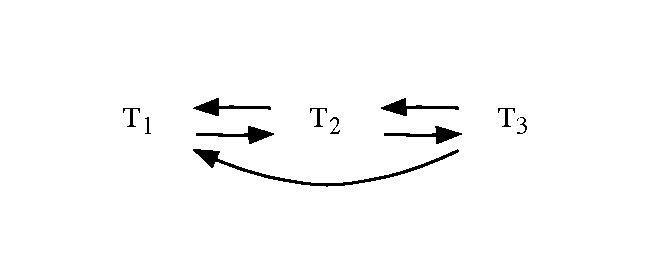
\includegraphics[]{task1_1} 
    \caption{conflict  serialization  graph }
    \label{}
\end{figure}

\clearpage
\subsection*{(2)}
\begin{table}[h]
    \centering
    \begin{tabular}{lll}
        \hline
        T1              & T2              & T3              \\ \hline
        lock(x) read(x) &                 &                 \\
        write(x, x+10)  &                 &                 \\
                        & lock(u) read(u) &                 \\
                        &                 & lock(y) read(y) \\
                        &                 & write(y, y+1)   \\
                        & lock(z) read(z) &                 \\
        read(z)         &                 &                 \\
        lock(z) wait    &                 &                 \\
                        & unlock(z)       &                 \\
        lock(z)         &                 &                 \\
        write(z, z+1)   &                 &                 \\
                        & lock(y) wait    &                 \\
                        &                 & unlock(y)       \\
                        & lock(y)         &                 \\
                        & write(y, z+2)   &                 \\
                        &                 & lock(v) read(v) \\
                        &                 & write(v, v+y)   \\
        lock(v) wait    &                 &                 \\
                        &                 & unlock(v)       \\
        lock(v)         &                 &                 \\
        write(v, v+z)   &                 &                 \\
                        & read(x)         &                 \\
        unlock(v)       &                 &                 \\
                        & unlock(y)       &                 \\
                        & unlock(u)       &                 \\
        unlock(z)       &                 &                 \\
        unlock(x)       &                 &                 \\ \hline
        \end{tabular}
        \end{table}
    
\clearpage
\subsection*{(3)}
\begin{table}[h]
    \centering
    \begin{tabular}{llll}
    \hline
    T1             & T2            & T3            & x                     \\ \hline
    timestamp(t1)  &               &               &                       \\
    read(x)        &               &               & x:t1                  \\
    write(x, x+10) &               &               &                       \\
                   & timestamp(t2) &               &                       \\
                   & read(u)       &               & u:t2                  \\
                   &               & timestamp(t3) &                       \\
                   &               & read(y)       & y:t3                  \\
                   &               & write(y, y+1) & y:t3                  \\
                   & read(z)       &               & z:t2                  \\
    read(z)        &               &               & z:t2:t1               \\
    write(z, z+1)  &               &               & z:t2:t1               \\
                   & write(y, z+2) &               & y:t3:t2 z:t2:t1:t2    \\
                   &               & read(v)       & v:t3                  \\
                   &               & write(v, v+y) & v:t3 y:t3:t2:t3       \\
    write(v, v+z)  &               &               & v:t3:t1 z:t2:t1:t2:t1 \\
                   & read(x)       &               & x:t1:t2               \\ \hline
    \end{tabular}
    \end{table}

\end{document}